\chapter{Background and Related Work}

This chapter will give some background about how Scratch works and why testing Scratch programs is a difficult task.
It will also highlight some related work, which has tackled to problem of testing Scratch programs.

\section{Scratch}

\begin{wrapfigure}{r}{0.35\textwidth + 5mm}
    \centering
    \vspace{-3mm}
    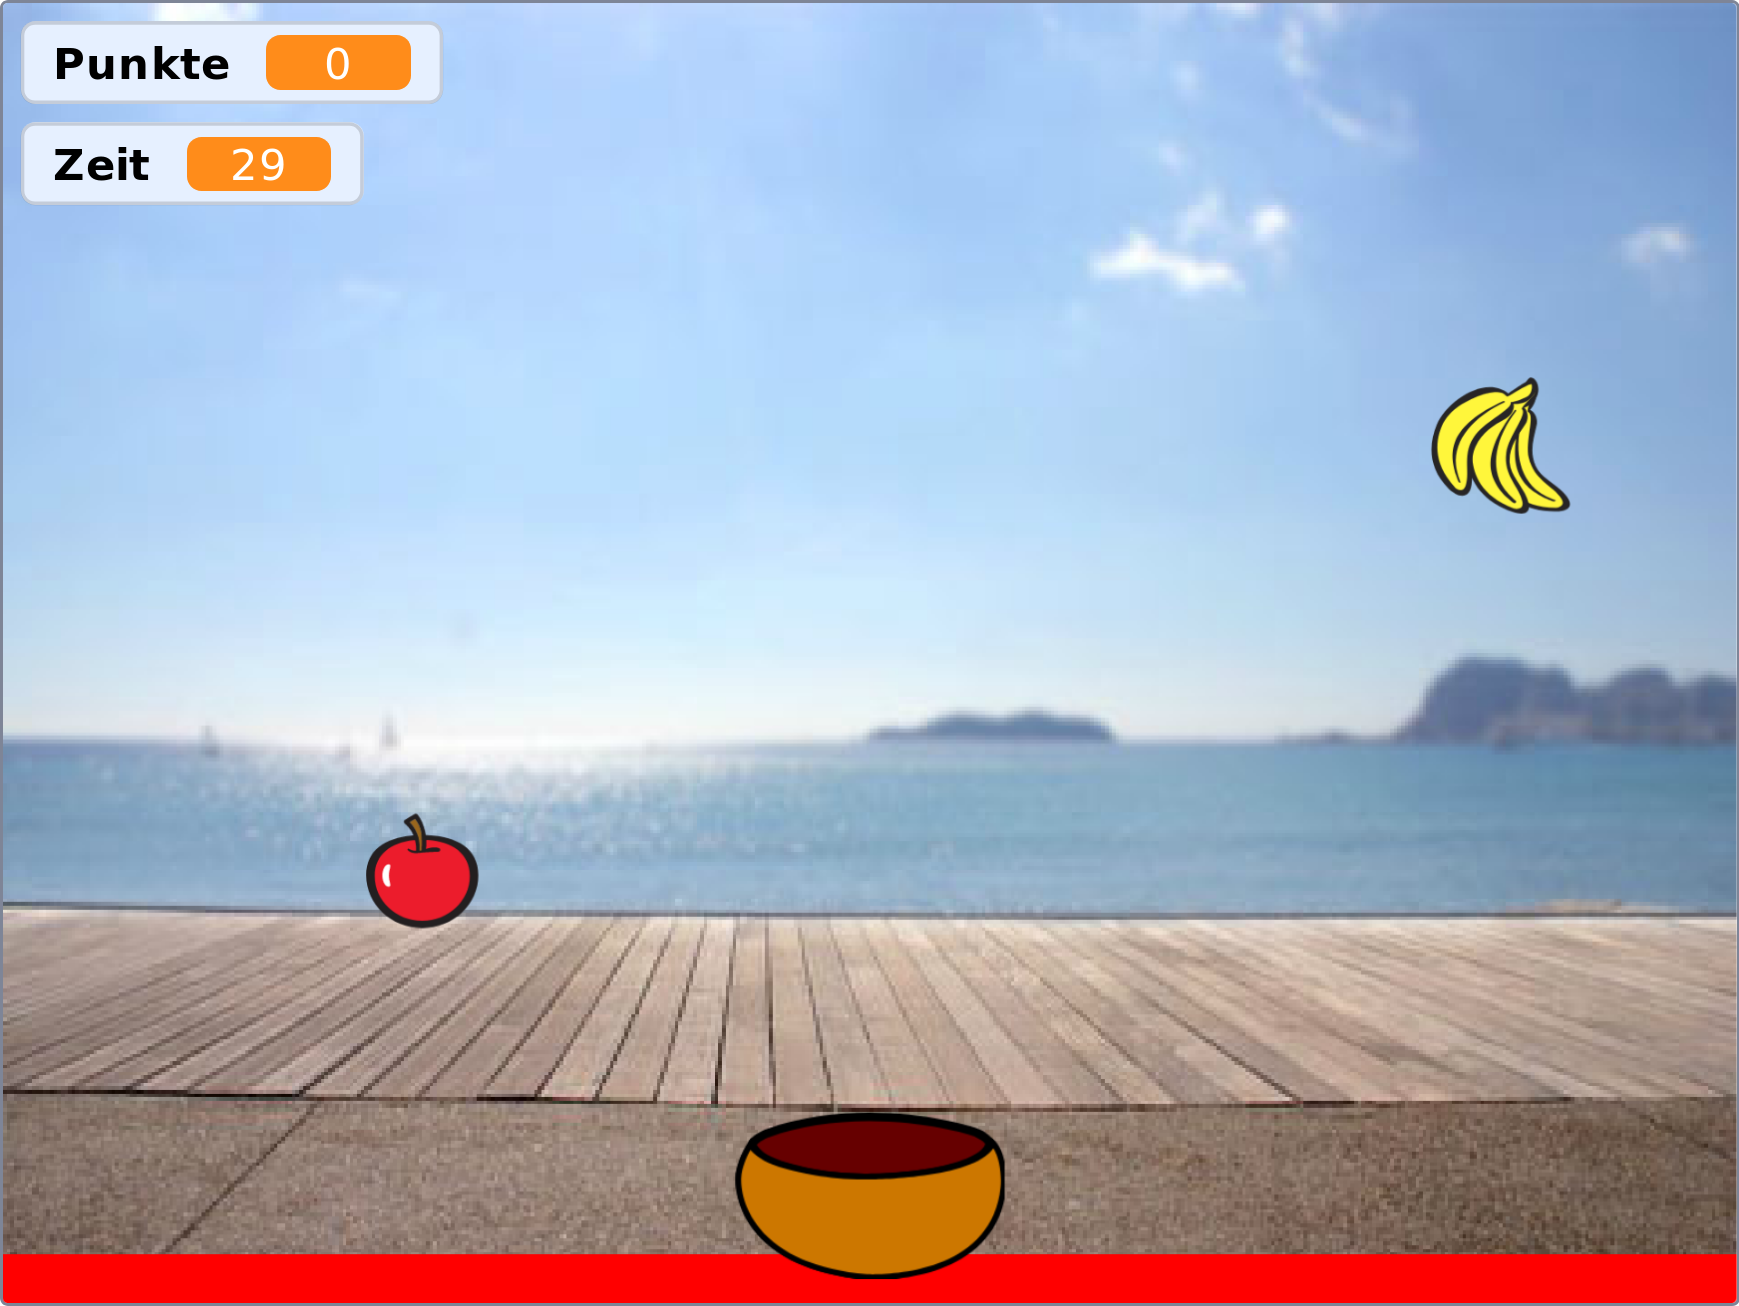
\includegraphics[width=0.35\textwidth]{scratch-stage}
    \caption{A catching game implemented in Scratch}
    \label{fig:a_catching_game_implemented_in_scratch}
\end{wrapfigure}
- Block based programming language developed by the MIT Media Lab~\cite{scratch}
- Aimed towards novices and children
- Block-based code eliminates the possibility of syntax errors
- Code creates interactive two-dimensional animations on a stage
- Possible to control the program with keyboard and mouse input, often creating game-like programs
    - Extensions offer more possibilities
- Heavily focused on multimedia, graphics and audio can easily be integrated into Scratch projects
\parspace

\begin{wrapfigure}{r}{0.45\textwidth + 5mm}
    \centering
    \vspace{-3mm}
    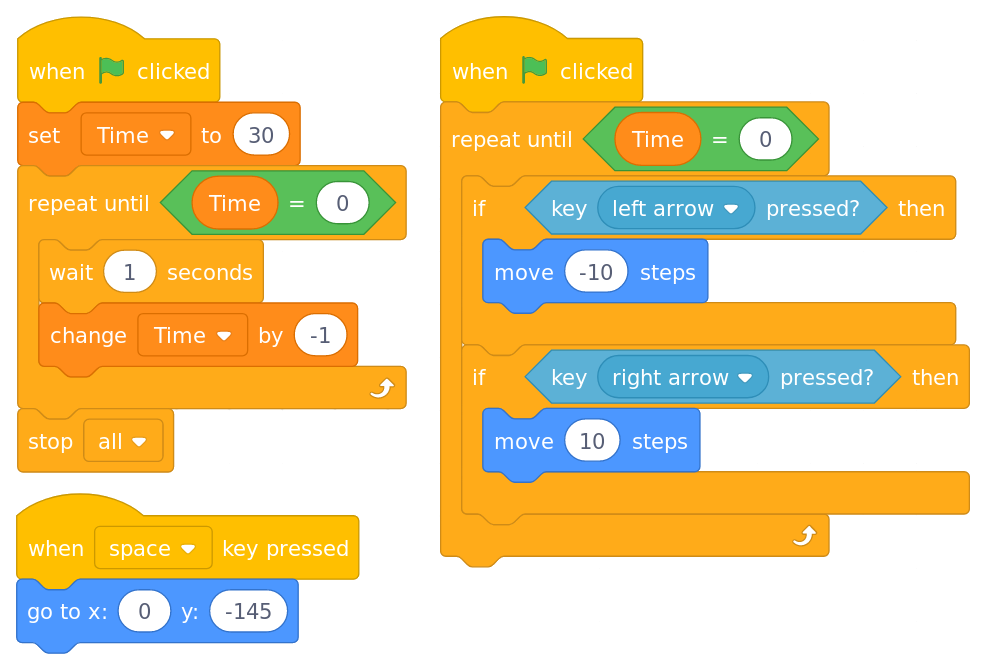
\includegraphics[width=0.45\textwidth]{scratch-code}
    \caption{Scratch blocks}
    \label{fig:scratch_blocks}
\end{wrapfigure}
- Code is made up by \textit{blocks}
- Multiple blocks combined together with a \textit{hat} make up a \textit{script}
- Scripts are called through their hats, they can be called by
    - input events, e.g. key press, mouse click
    - other scripts and sprites through by broadcasting messages
    - green flag, the program is started through the green flag

- All currently running scripts conceptually run in parallel
- Scratch VM sequentializes $\rightarrow$ no race conditions on the language level
\parspace

\begin{wrapfigure}{r}{0.45\textwidth + 5mm}
    \centering
    \vspace{-4mm}
    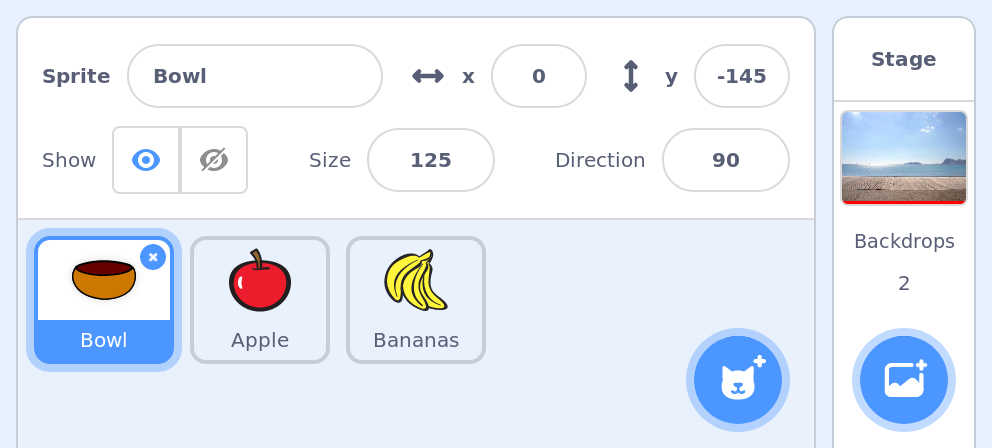
\includegraphics[width=0.45\textwidth]{scratch-sprites}
    \caption{The sprite menu}
    \label{fig:the_sprite_menu}
\end{wrapfigure}
- Visual objects are represented as sprites
- The code of the program is split between the sprites
- Each sprite and the stage have their own code which manipulates them and can interact with the code of other sprites
- Sprites have variables, which they can access
- Every sprite can access the stage's variables
\parspace

% \begin{wrapfigure}{r}{0.25\textwidth + 5mm}
%     \centering
%     \vspace{-3mm}
%     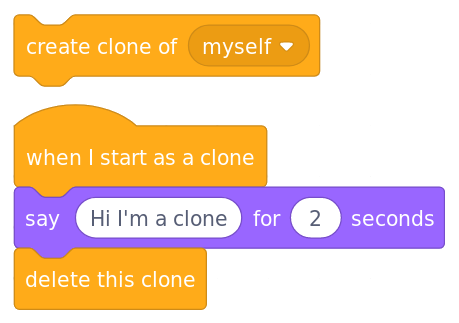
\includegraphics[width=0.25\textwidth]{scratch-code-clone}
%     \caption{Creating clones}
%     \label{fig:creating_clones}
% \end{wrapfigure}
% - To create a second instance of a sprite, a sprite can clone itself
% - The new sprite then runs scripts that have a ''when I start as a clone'' hat
% - The new clone accesses the same variables as the original sprite, variables are not copied
% \parspace
%
% Lorem ipsum dolor sit amet, consectetur adipiscing elit. Etiam cursus neque at magna vehicula, id lobortis massa tempus. Ut vitae orci euismod, posuere purus at, fringilla justo. Suspendisse in sodales neque. Mauris odio enim, varius sed porttitor in, ullamcorper nec eros. Aenean placerat arcu non leo imperdiet sodales. Nullam vestibulum justo nibh. Duis ac nibh congue, molestie sapien in, condimentum turpis. Donec in nisl vitae sem vehicula vehicula ac non velit. Integer at laoreet sapien. Lorem ipsum dolor sit amet, consectetur adipiscing elit. Aliquam suscipit arcu condimentum rhoncus auctor. Donec porta augue vitae quam malesuada posuere.

\section{Previous Testing Approaches}

- Since the multimedia nature of Scratch programs makes testing Scratch programs difficult,
  automatic assessment of Scratch programs is still an open problem
- At least two other projects have tackled the task of automatically assessing Scratch projects.

=== Hairball
- Hairball \cite{hairball} allows static analysis of scratch programs
- Written in Python
- Takes the source file of a scratch project and performs static analysis
- Has a plugin-based architecture
    - Comes with pre-defined plugins, for example to detect dead code or wrong synchronization between broadcast blocks and their receivers
    - allows to define own plugins, which iterate over the scratch blocks to analyze them
- Possible use cases:
    - check if students use a new construct, which the exercise focuses on
    - detect code smells
    - measure the complexity of a program $\rightarrow$ see Dr.Scratch
- Since it only allows static analysis, not suitable to check the functionality of a program
- Already used in DrScratch \cite{drscratch} to automatically determine the complexity of Scratch programs.

=== ITCH
- ITCH (Individual Testing of Computer Homework for Scratch Assignments)~\cite{itch}
- set of Python scripts
- allows simple textual input-output testing with pre-defined values using "ask" and "say" blocks
- Works by replacing "ask" and "say" blocks in the project
    - "ask" and "say" blocks are used in Scratch to ask the user for textual input and to display textual output on the screen
      (use cartoon speech bubbles)
    - "ask" blocks are replaced by configured test input
    - "say" blocks save the value into a variable instead of displaying it
    $\rightarrow$ the value can then be retrieved by saving the project and reading the value from the saved project
    - TODO picture of say and ask blocks
- This, however, only allows to test projects with a small subset of Scratch functionality
- Only useful for very specific tasks that don't have much to do with Scratch's strengths
- Not very useful in general for Scratch because it focuses on multimedia and creativity
- Other languages are better suited for this task: BlockPy~\cite{blockpy}
    - Has similar operators
    - Provides a way to convert the block constructs to Python code, which can be automatically tested easily

\section{Challenges of Testing Scratch Programs}
- Runtime testing of Scratch programs has some caveats
- This section explains some critical details that make testing of Scratch programs difficult

=== Parallel scripts
- Individual testing of program parts problematic
    - Scratch runs multiple scripts in parallel
        - Scripts often depend on one another
    - Not very useful to test single program parts
    - Possible to define multiple independent scripts that each activate with a different button press
        - but becomes convoluted
        - but defeats to purpose of Scratch to create a interactive environment
$\rightarrow$ Use a complete black box approach
    - Scratch programs are controlled by simulating user input instead of manually calling certain scripts
    - The only information, which is checked, is what appears on screen
        - properties of sprites and variables

=== Lack of IO, multimedia nature
- Scratch has a Lack of traditional IO mechanisms
    - makes it hard to extract information about the current program state
    - makes it hard to control the execution of a Scratch program
    - no traditional input output testing possible without limiting the project to a small subset of Scratch's functionality
$\rightarrow$ Give test cases an interface that can be used to interact with the Scratch project
    - interacts directly with the Scratch virtual machine
    - a way to get information about sprites and variables
    - a way to simulate user input

=== Many tested properties will depend on time
- A tested property might depend on a previous value
    - e.g. check if a sprite is moving right
    - sprites save the values from the previous execution step
- Some tested properties should hold for a time or for the whole execution
    - Provide a way to define constraints that must always hold

\section{Black Box Testing}

- Black box approach:
    - Block box testing bases tests on the specification of the tested program
    - Tests are written without knowledge of the internals of a program
    - Program is seen as a ''black box'' that takes some input and produces some output.
    - Program specification is in the case of Scratch programs most likely a task description for some course or tutorial

    - Input for the black box is user interaction through mouse and keyboard
    - Interact only how a user can interact with the program
        - Since Scratch can only be controlled through user interaction and has no API to call blocks or scripts,
          it only makes sense to control the program this way in the test
        - No information about the internals of the program other than sprite and variable names
            - Sprite names should be included in the specification so the test can more easily identify sprites
            - Giving no or little information about the implementation makes sense for a task description
    - Output of the black box are changes on Scratch's stage
    - Test only what the user sees
        - Only information about sprites and variables (both can be shown on screen)
        - Sprite positions, movement, looks, etc.

\section{Automatic Test Generation}%
\label{sec:automatic_test_generation}

